\documentclass[a4paper,12pt]{article}
\usepackage[slovene]{babel}
\usepackage[utf8]{inputenc}
\usepackage[T1]{fontenc}
\usepackage[a4paper, total={16cm, 22cm}]{geometry}
\usepackage{lmodern}
\usepackage{amsmath,amsfonts}
\usepackage{amsthm}
\usepackage{setspace}
\usepackage{mathtools}

\def\N{\mathbb{N}}
\def\Z{\mathbb{Z}}
\def\Q{\mathbb{Q}}
\def\R{\mathbb{R}}

\theoremstyle{definition}
\newtheorem{definicija}{Definicija}
\newtheorem{zgled}{Zgled}
\theoremstyle{plain}
\newtheorem{izrek}{Izrek}
\newtheorem{lema}{Lema}
\newtheorem{trditev}{Trditev}
\newtheorem{posledica}{Posledica}

\newenvironment{dokaz}{\begin{proof}[\bfseries\upshape\proofname]}{\end{proof}}

\DeclarePairedDelimiter\ceil{\lceil}{\rceil}
\DeclarePairedDelimiter\floor{\lfloor}{\rfloor}

\newcommand{\geslo}[2]{\noindent \textbf{#1} \quad #2 \hfill \break}

\setstretch{1.2}

\title{Porazdelitev praštevil}
\author{Matevž Miščič}
\date{21. avgust 2023}



\begin{document}

\maketitle{}

\section{Uvod}
Praštevila so v matematiki pomembna, saj so gradniki vseh naravnih števil. Velja namreč, da lahko vsako naravno število, večje od $1$, zapišemo kot produkt praštevil. Poleg matematike so praštevila pomembna tudi v računalništvu, še posebej v kriptografiji. V tej predstavitvi si bomo ogledali nekaj zanimivih rezultatov o porazdelitvi praštevil.



\section{Praštevila}

Začnimo z definicijo.

\begin{definicija}
    \emph{Praštevilo} je naravno število, ki ima natanko dva delitelja.
    Naravno število, ki ima vsaj tri delitelje, imejujemo \emph{sestavljeno število}.
\end{definicija}
Prvih nekaj praštevil je $2, 3, 5, 7, 11, 13, \ldots$. Število $6$ je sestavljeno število, ker ima štiri delitelje: $1, 2, 3, 6$.

Naslednja lastnost praštevil je ključnega pomena.

\begin{trditev}
    \label{factorisation}
    Vsako naravno število, večje od $1$, se da zapisati kot produkt števil.
\end{trditev}
\begin{dokaz}
    Trditev bomo pokazali z indukcijo. Naj bo $n$ naravno število, ki je večje od $1$. Če sta $1$ in $n$ edina delitelja števila $n$, je $n$ praštevilo in ni kaj dokazati. Sicer obstaja nek delitelj $a$ števila $n$, da velja $1 < a < n$. Torej je $n = ab$ za nek $b \in \N$. Ker je $1 < a, b < n$ lahko po indukcijski predpostavki $a$ in $b$ zapišemo kot produkt praštevil, zato enako velja za njun produkt $n$.
\end{dokaz}

Posledica te trditve je, da je praštevil neskončno mnogo. To je rezultat, ki ga je poznal že Evklid okoli leta 300 pred našim štetjem.

\begin{posledica}
    Praštevil je neskončno mnogo.
\end{posledica}
\begin{dokaz}
    Recimo, da jih je le končno mnogo. Naj bodo $p_1, p_2, \ldots, p_k$ vsa praštevila. Vzemimo $n = p_1p_2 \cdots p_k + 1$. Po prejšnji trditvi vemo, da lahko $n$ zapišemo kot produkt praštevil, ampak očitno nobeno od praštevil ne deli $n$, torej smo prišli v protislovje.
\end{dokaz}



\section{Praštevilski izrek}
Zanima nas, kako gosta so praštevila med naravnimi števili. Intuitivno se nam zdi, da praštevila postajajo vedno manj gosta. Na primer, med $1$ in $100$ je $25$. praštevil, med $1001$ in $1100$ pa samo $16$. Razlog za to je, da je naravno število $n$ praštevilo natanko tedaj, ko ni deljivo z nobenim praštevilom manjšim od $n$. Za večje $n$ torej obstaja več praštevil, ki ne smejo deliti $n$, zato je manj verjetno, da je $n$ praštevilo.

Poskusimo formalizirati prejšnje ideje.
\begin{definicija}
    Za naravno število $n \in \N$ s $\pi(n)$ označimo število praštevil manjših ali enakih $n$.
\end{definicija}
Zanima nas, kako raste funkcija $\pi$. Zgornja intuicija pravi, da raste vedno počasneje.

\begin{izrek}[Čebišov]
    Obstajata pozitivni realni števili $A, B > 0$, da za vsak $n \in \N$ velja $$A\frac{n}{\log{n}} < \pi(n) < B\frac{n}{\log{n}}.$$
\end{izrek}

Po izreku Čebišova torej, funkcija $\pi$ raste približno tako hitro kot funkcija $\frac{n}{\log{n}}$. Velja pa še veliko več, kar pove naslednji izrek.

\begin{izrek}[Praštevilski izrek]
    Velja $$\lim_{n \rightarrow \infty} \frac{\pi(n)}{n / \log{n}} = 1.$$
\end{izrek}

\begin{center}
    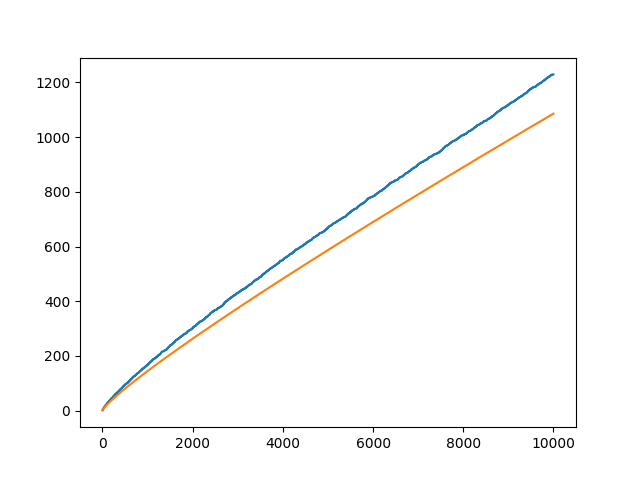
\includegraphics[scale=0.8]{graf1.png}
\end{center}

Ta izrek je netrivialen in ga ne bomo dokazali. Precej lažje je dokazati izrek Čebišova, a bomo tudi tega izpustili. Bomo pa kasneje videli dokaz Bertrandovega postulata, ki uporablja podobne metode.

Posledica praštevilskega izreka je, da obstaja približno $\frac{n}{\log{n}}$ praštevil, ki so manjša od $n$. Verjetnost, da je naključno izbrano število med $1$ in $n$ praštevilo, je torej približno $\log{n}$.




\section{Praštevila v aritmetičnih zaporedjih}
Vemo že, da je praštevil neskončno. Za dano aritmetično zaporedje $an + b$, kjer sta $a, b, \in \N$, se lahko vprašamo, ali je neskončno mnogo praštevil med členi tega zaporedja. Če si $a$ in $b$ nista tuja, imata skupni delitelj $d > 1$, ki deli vse člene zaporedja, zato v zaporedju ni neskončno praštevil. Predpostavimo torej, da sta si $a$ in $b$ tuja. Velja naslednji izrek.

\begin{izrek}[Dirichlet]
    Naj bosta $a, b \in \N$ tuji si števili. Potem je med členi zaporedja $an + b, n \in \N$ neskončno praštevil.
\end{izrek}

\begin{zgled}
    Če je $a = 3$ in $b = 6$, dobimo aritmetično zaporedje $9, 12, 15, 18, 21, 24, \ldots$. V tem zaporedju so vsi členi deljivi s $3$, ki je največji skupni delitelj $a$ in $b$.
    
    Če je $a = 8$ in $b = 3$, dobimo zaporedje $11, 14, 17, 20, 23, 26, 29, \ldots$. Od tega so $11, 17, 23, 29$ praštevila. Po Dirichletovem izreku obstaja neskončno praštevilskih členov tega zaporedja.
\end{zgled}

Tudi tega izreka ne bomo dokazali, bomo pa pokazali enostaven primer, ko je $a = 6$ in $b = 5$.

\begin{trditev}
    Med števili oblike $6n + 5$ je neskončno praštevil.
\end{trditev}
\begin{dokaz}
    Naj bo $p > 3$ poljubno praštevilo in $q = 2 \cdot 3 \cdot 5 \cdots p - 1$. Vsako praštevilo, ki je večje od $3$, je oblike $6n + 1$ ali pa oblike $6n + 5$. Očitno je $q$ oblike $6n + 5$. Vsi prafaktorji $q$ ne morejo biti oblike $6n + 1$, saj bi potem tudi $q$ bil take oblike. Torej obstaja prafaktor $q$, ki je oblike $6n + 5$ in je seveda večji od $p$. Torej obstaja neskončno praštevil take oblike.
\end{dokaz}

Podoben dokaz deluje tudi za $a = 4$ in $b = 3$.



\section{Razmaki med praštevili}
Raliki dveh zaporednih praštevil pravimo razmak med praštevili. Najprej bomo pokazali, da obstajajo poljubno veliki razmaki med praštevili.

\begin{trditev}
    Obstajajo poljubno veliki bloki zaporednih naravnih števil, ki so vsa sestavljena števila.
\end{trditev}
\begin{dokaz}
    Naj bo $n \in \N$. Števila $n! + 2, n! + 3, n! + 4, \ldots, n! + n$ so deljiva z $2, 3, \ldots, n$, zato so vsa sestavljena.
\end{dokaz}

Po praštevilskem izreku je povprečen razmak med preštevili manjšimi od $n$ približno $\log{n}$. Razmaki torej postajajo vse večji.

V zvezi z razmaki bomo spoznali še Bertrandov postulat in nerešeno domnevo o praštevilskih dvojčkih.

\subsection{Domneva o praštevilskih dvojčkih}
Praštevilski dvojček je par praštevil $(p, q)$, za katerega velja $q - p = 2$. Primeri praštevilskih dvojčkov so $(3, 5), (5, 7), (9, 11), (11, 13)$. Domneva o praštevilskih dvojčkih sprašuje, če obstaja neskončno praštevilskih dvojčkov. Domneva je še vedno nerešena, a matematiki verjamejo, da je odgovor pritrdiln.

Leta 2013 je Yitang Zhang dokazal, da obstaja naravno število $n < 70 \cdot 10^6$, za katerega obstaja neskončno parov praštevil z razliko $n$. Približno leto kasneje so matematiki to število uspeli zmanjšati na $246$.






\section{Bertrandov postulat}
Naslednji rezultat o porazdelitvi praštevil je Bertrandov postulat, ki pravi, da ne obstajajo prevelike luknje med zaporednima prašteviloma. Izrek je prvi dokazal Pafnuti Čebišov leta 1850, mi pa si bomo ogledali enostavnejši dokaz, ki ga je podal Paul Erd\H{o}s leta 1932.

\begin{izrek}
    Za vsako naravno število $n \in \N$ obstaja praštevilo $p$ za katero velja $n \leq p \leq 2n$.
\end{izrek}


\subsection{Paul Erd\H{o}s}
Paul Erd\H{o}s je bil Madžarski matematik, ki je živel od leta 1913 do 1996. Je eden od najplodnejših matematikov 20. stoletja. Ukvarjal se je predvsem z reševanjem nerešenih problemov, ne pa z razvijanjem novih teorij. Večino svojega časa je potoval med znanstvenimi konferencami in kolegi s katerimi je tudi znanstveno sodeloval, kar je razvidno tudi iz njegovega citata: ">Another roof, another proof."< Po smrti svoje mame je začel jemati Amfetamin. Njegov zaskrbljen prijatelj Ron Graham je z njim stavil, da ne more nehati jemati droge za en mesec. Erd\H{o}s je stavo zmagal, se pa je prioževal nad svojo neproduktivnostjo v tem mesecu in rekel, da zaradi Rona matematika zaostaja za en mesec.


\subsection{Dokaz Bertrandovega postulata}
Izrek bomo dokazali s podrobno analizo tega, katera praštevila delijo centralne binomske koeficiente.

\begin{definicija} % povej kaj je fakulteta
    Centralni binomski koeficient je število $$C_n = \binom{2n}{n} = \frac{(2n)!}{n!^2}.$$
\end{definicija}

\begin{lema}
    \label{lema1}
    Za vsako naravno število $n$ velja $\frac{4^n}{2n} \leq C_n$.
\end{lema}
\begin{dokaz} % ponovi binomski izrek
    Velja $$4^n = (1+1)^{2n} = \sum_{k = 0}^{2n} \binom{2n}{k} = 2 + \sum_{k = 1}^{2n - 1} \binom{2n}{k} \leq 2 + (2n - 1)\binom{2n}{n} \leq 2n\binom{2n}{n}.$$
\end{dokaz}

\begin{lema}
    \label{lema2}
    Za vsako naravno število $n \in \N$ za praštevilski razcep $C_n = p_1^{a_1} \cdots p_r^{a_r}$ velja $p_i^{a_i} \leq 2n$ za vsak $i = 1,\ldots,r$. 
\end{lema}
\begin{dokaz}
    Največjo naravno število $a$, da $p^a$ deli $m$, označimo s $\nu_p(m)$. Velja $$\nu_p(n!) = \floor*{\frac{n}{p}} + \floor*{\frac{n}{p^2}} + \floor*{\frac{n}{p^3}} + \cdots.$$ Sledi $$\nu_p(C_n) = \nu_p((2n)!) - 2\nu_p(n!) = \left( \floor*{\frac{2n}{p}} - 2\floor*{\frac{n}{p}} \right) + \left( \floor*{\frac{2n}{p^2}} - 2\floor*{\frac{n}{p^2}} \right) + \cdots.$$ Za vsak $k$ velja $$0 \leq \floor*{\frac{2n}{p^k}} - 2\floor*{\frac{n}{p^k}} \leq 1,$$ za $k$ tak, da je $p^k > 2n$, pa je $\floor*{\frac{2n}{p^k}} - 2\floor*{\frac{n}{p^k}} = 0$. Sledi $p_i^{a_i} \leq 2n$ za vse $i$.
\end{dokaz}

\begin{lema}
    \label{lema3}
    Za vsako naravno število $n \in \N$ in praštevilo $p \neq 2$ z $\frac{2n}{3} < p < n$ velja, da $p$ ne deli $C_n$. 
\end{lema}
\begin{dokaz}
    Za $n \leq 4$ je trditev očitna. Recimo torej, da je $n \geq 5$. Z dokaza prejšnje leme vemo $$\nu_p(C_n) = \left( \floor*{\frac{2n}{p}} - 2\floor*{\frac{n}{p}} \right) + \left( \floor*{\frac{2n}{p^2}} - 2\floor*{\frac{n}{p^2}} \right) + \cdots.$$ Ker je $\frac{2n}{3} < p < n$, je $1 < \frac{n}{p} < \frac{3}{2}$, zato je $\floor*{\frac{2n}{p}} = 2\floor*{\frac{n}{p}} = 2$ in $\floor*{\frac{2n}{p}} - 2\floor*{\frac{n}{p}} = 0$. Potem za $k \geq 2$ velja $p^k \geq p^2 > (\frac{2n}{3})^2 = \frac{4}{9}n^2 > 2n$, kjer smo v zadnji neenakosti upoštevali $n \geq 5$. Sledi $\floor*{\frac{2n}{p^k}} - 2\floor*{\frac{n}{p^k}} = 0$, torej je $\nu_p(C_n) = 0$ oziroma $p$ ne deli $C_n$.
\end{dokaz}

\begin{definicija}
    Za naravno število $n \in \N$ definirajmo $n$-to primorielo kot produkt vseh praštevil manjših ali enakih $n$ in jo označimo z $n\#$.
\end{definicija}

\begin{lema}
    \label{lema4}
    Za vsako naravno število $n \in \N$ velja $n\# < 4^n$. 
\end{lema}
\begin{dokaz}
    Trditev bomo dokazali z indukcijo. Za $n = 1, 2$ očitno velja. Naj bo torej $n \geq 3$. Če $n$ ni praštevilo, potem je $n\# = (n - 1)\# < 4^{n - 1} < 4^n$ po indukcijski predpostavki. Če je $n$ praštevilo, je $n$ lih, zato je $n = 2m + 1$ za nek $m \in \N$.
    
    Vsa preštevila med $m + 2$ in $2m + 1$ delijo $\binom{2m + 1}{m}$, torej $\frac{(2m + 1)\#}{(m + 1)\#}$ deli $\binom{2m + 1}{m}$.

    \begin{align*}
        \binom{2m + 1}{m} <& \binom{2m + 1}{0} + \cdots + \binom{2m + 1}{m} = \frac{1}{2} \left( \binom{2m + 1}{0} + \cdots + \binom{2m + 1}{2m + 1} \right)\\ =& \frac{1}{2} 2^{2m + 1} = 4^m.
    \end{align*}

    Torej $\frac{(2m + 1)\#}{(m + 1)\#} < 4^m$. Po indukcijski predpostavki je $(m + 1)\# < 4^{m + 1}$, zato je $$n\# = (2m + 1)\# < 4^m (m + 1)\# < 4^m 4^{m + 1} = 4^{2m + 1} = 4^n.$$
\end{dokaz}

\begin{dokaz}
    Recimo, da obstaja tak $n \in \N$, da ni praštevila $p$, za katerega bi veljalo $n \leq p \leq 2n$. Oglejmo si praštevilski razcep $C_n$. Očitno so vsi prafaktorji manjši ali enaki $2n$. Ker ni preštevil med $n$ in $2n$, so vsi celo manjši od $n$. Po lemi \ref{lema3} noben prafaktor $C_n$ ni med $\frac{2n}{3}$ in $n$, zato so vsi prafaktorji manjši ali enaki $\frac{2n}{3}$.

    Recimo, da je $n \geq 5$ in torej velja $\sqrt{2n} < \frac{2n}{3}$. Zapišemo lahko $C_n = P_1 P_2$, kjer je $P_1$ produkt prafaktorjev, ki so manjši ali enaki $\sqrt{2n}$, $P_2$ pa produkt prafaktorjev med $\sqrt{2n}$ in $\frac{2n}{3}$. Naj bo $P_1 = p_1^{a_1} \cdots p_k^{a_k}$ in $P_2 = q_1^{b_1} \cdots q_l^{b_l}$. 
    
    Po lemi \ref{lema2} za vse $i = 1, \ldots, k$ velja $p_i^{a_i} < 2n$, zato je $P_1 < (2n)^k \leq (2n)^{\sqrt{2n}}$. Ker za $i = 1, \ldots, l$ velja $q_i^{b_i} \leq 2n$ in $q_i > \sqrt{2n}$, mora veljati $b_i = 1$ za vse $i$. 
    
    Z uporabo leme \ref{lema4} dobimo oceno $P_2 = q_1 \cdots q_l \leq (\frac{2n}{3})\# < 4^\frac{2n}{3}$. 
    
    Iz leme \ref{lema1} sledi $\frac{4^n}{2n} \leq C_n = P_1 P_2 < (2n)^{\sqrt{2n}} 4^{\frac{2n}{3}}$, kar velja le za $n \leq 467$. Za $n \geq 468$ smo torej pokazali, da mora obstajati praštevilo med $n$ in $2n$. Da to velja tudi za $n \leq 467$ pokažemo z zaporedjem praštevil $2, 3, 5, 7, 13, 23, 43, 83, 163, 317, 631$, v katerem je vsako naslednje manjše od dvakratnika prejšnjega.
\end{dokaz}



\begin{thebibliography}{1}
    \bibitem{1}
    J.~A.~Hocutt in P.~L.~Robinson, \emph{Everywhere Differentiable, Nowhere Continuous Functions}, Amer.~Math.~Monthly \textbf{125} (2018) 923--928.
    \bibitem{2}
    P.~R.~Halmos, \emph{Problems for Mathematicians, Young and Old}, Dolciani Mathematical Expositions \textbf{12}, Mathematical Association of America, Washington, 1991.
\end{thebibliography}


\end{document}